\documentclass{standalone}

\usepackage[utf8]{inputenc}
\usepackage{amsfonts}
\usepackage{amssymb,amsmath}
\usepackage{tikz}
\usetikzlibrary{shapes,decorations.pathreplacing}

\begin{document}

\begin{large}
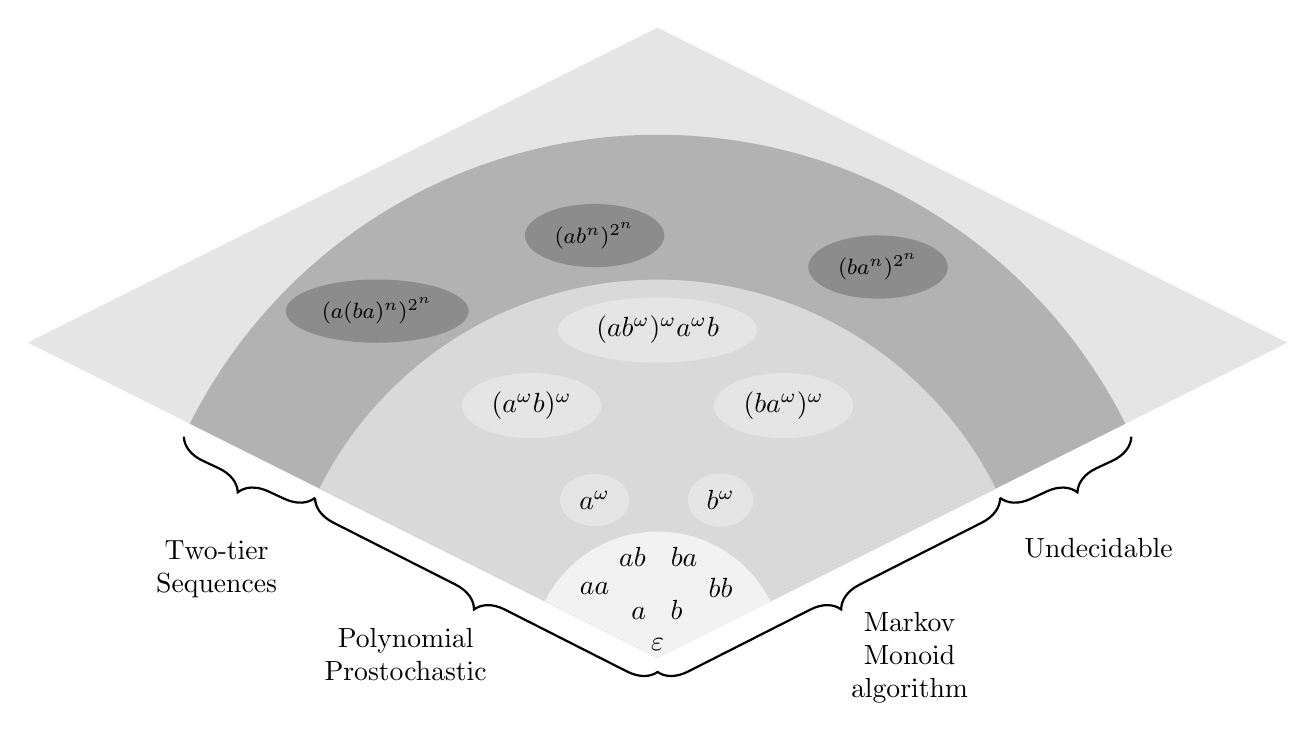
\begin{tikzpicture}[scale=.8]
%\draw (-10,0) grid (10,10);

\draw [thick, decorate,decoration={brace,amplitude=10pt}, rotate=65] (-.2,-.1) -- (0,6) ;
\draw (-4,0) node {\begin{tabular}{c}Polynomial\\ Prostochastic\end{tabular}};

\draw [thick, decorate,decoration={brace,amplitude=10pt}, rotate=65] (0,6) -- (0,8.3) ;
\draw (-7,1.4) node {\begin{tabular}{c}Two-tier\\ Sequences\end{tabular}};

\draw [thick, decorate,decoration={brace,amplitude=10pt,mirror}, rotate=-65] (.2,-.1) -- (0,6) ;
\draw (4,0) node {\begin{tabular}{c}Markov\\ Monoid\\ algorithm\end{tabular}};

\draw [thick, decorate,decoration={brace,amplitude=10pt,mirror}, rotate=-65] (0,6) -- (0,8.3);
\draw (7,1.7) node {\begin{tabular}{c}Undecidable\end{tabular}};

\clip (0,0) -- (-10,5) -- (0,10) -- (10,5) -- (0,0);

\fill[gray!20] (-10,0) rectangle (10,10);
\fill[gray!60] (0,0) circle (8.3);
\fill[gray!30] (0,0) circle (6);
\fill[gray!10] (0,0) circle (2);

\draw (0,.2) node {$\varepsilon$} ;
\draw (-.3,.7) node {$a$} ;
\draw (.3,.75) node {$b$} ;
\draw (-1,1.1) node {$aa$} ;
\draw (-.4,1.6) node {$ab$} ;
\draw (.42,1.6) node {$ba$} ;
\draw (1,1.1) node {$bb$} ;

\node [ellipse,fill=gray!20] at (-1,2.5) {$a^\omega$} ;
\node [ellipse,fill=gray!20] at (1,2.5) {$b^\omega$} ;
\node [ellipse,fill=gray!20] at (-2,4) {$(a^\omega b)^\omega$} ;
\node [ellipse,fill=gray!20] at (2,4) {$(b a^\omega)^\omega$} ;
\node [ellipse,fill=gray!20] at (0,5.2) {\begin{normalsize}$(a b^\omega)^\omega a^\omega b$\end{normalsize}} ;

\node [ellipse,fill=gray!90] at (-4.45,5.5) {\begin{footnotesize}$(a (ba)^n)^{2^n}$\end{footnotesize}} ;
\node [ellipse,fill=gray!90] at (-1,6.7) {\begin{footnotesize}$(a b^n)^{2^n}$\end{footnotesize}} ;
\node [ellipse,fill=gray!90] at (3.5,6.2) {\begin{footnotesize}$(b a^n)^{2^n}$\end{footnotesize}} ;
\end{tikzpicture}
\end{large}

\end{document}